\lecture{2}{2025-09-18}{}{}
\begin{parag}{Catastrophic cancellation}
    Of all the mathematical operations, one particular case is \important{especially dangerous}
    \begin{align*} a - b \mathspace \left(a \approx b\right) \end{align*}
    The also happens for $a + b$ when $a \approx -b$ This can lead to catastrophic cancellation even if the substraction is done without error (this can happend not only if the there is an rounding error in the operation but maybe from before).
    \begin{subparag}{Example}
        For instance $3.140 = 2^1 \cdot 1.10010010$ and $-3.149 = + 2^1 1.10010010$
	When you sum both you get:
	\begin{align*} = -2^{-7} 1.0_2 \end{align*}
    \end{subparag}
\end{parag}


\begin{parag}{Quantiying error}
    \begin{itemize}
	    \item Absolute error: $\left|\text{true value} - \text{aprroximate value}\right|$
		    \begin{itemize}
			    \item Example 2cm $\pm 0.1 cm$
		    \end{itemize}
	    \item Relative error: $\frac{\text{absolute error}}{\left|\text{true value}\right|}$
		    \begin{itemize}
			    \item Example: 2cm $\pm 0.1 \%$
			    \item Another common notation (true value) (1 $\pm $relative error)
		    \end{itemize}
		    
    \end{itemize}
    
\end{parag}
\begin{parag}{Forward ans Backward Error}
	\begin{center}
	\includegraphics[scale=0.3]{screenshots/2025-11-28_1.png}
	\end{center}
    \begin{subparag}{Example}
        For instance let us take
	\begin{align*} f(x) := \sqrt{x} \\
	y =  f(x)\\
\bhat{y} = f_{IEE754}(x)\end{align*}
    \end{subparag}
    Here is you wanted to compute the the backward error you would do it like this:
    \begin{align*} error = x - \left(f_{IEE754}(x)\right)^2 \end{align*}
\end{parag}
\begin{parag}{Conditioning of numerical problems}
   \begin{center}
   \includegraphics[scale=0.3]{screenshots/2025-11-28_2.png}
   \end{center} 
   \begin{align*} \text{condition number: ratio} \frac{\text{forward error}}{\text{backward error}}\end{align*}
\end{parag}

\section{Linear systems}

\begin{definition}
$f$ is a linear function if and only if:
\begin{itemize}
	\item $f\left(x, y\right) =  f\left(x\right) + f\left(y\right)$ \hfill additivity
	\item $f\left(\alpha x\right) =  \alphaf\left(x\right) $ where $\alpha \in \mathbb{R}$ \hfill homogeneity
\end{itemize}
In this case $f\left(x\right) = Ax$ fully encodes everything that $f$ does!

\end{definition}

\begin{parag}{Geometric intrerpretation of matrix-vector product}
	\begin{align*} \left(Ax\right)_i = \sum_{k= 1}^{n}A_{ik}x_k \text{ where } A = \begin{pmatrix} \mid & \mid & \mid \\ a^{\left(1\right)} & a^{\left(2\right)} & a^{\left(3\right)}\\ \mid & \mid & \mid \end{pmatrix}  \end{align*}
Example of linearly dependent columns span 2d Subspace:
\begin{align*} Ax = a^{(1)}x_1 + a^{(2)}x_2 + a^{(3)}x_3 \end{align*}
\begin{center}
\includegraphics[scale=0.15]{screenshots/2025-11-28_3.png}
\end{center}    
\end{parag}



\begin{parag}{Basic matric transformation in 2D}
	Please see the video of 3blue1brown on essence of linear algebra to understand this well
\end{parag}

\begin{figure}[h!]
\centering

\begin{subfigure}{0.48\textwidth}
    \centering
    \textbf{Scaling}\par
	    \begin{align*} \begin{pmatrix} v_x' \\ v_y' \end{pmatrix} = \begin{pmatrix} 2 & 0 \\ 0 & 2 \end{pmatrix} \begin{pmatrix} v_x \\ v_y \end{pmatrix}  \end{align*}
    \includegraphics[width=\linewidth]{screenshots/2025-11-28_5.png}
\end{subfigure}
\hfill
\begin{subfigure}{0.48\textwidth}
    \centering
    \textbf{Shear}\par
	    \begin{align*} \begin{pmatrix} v_x' \\ v_y' \end{pmatrix} = \begin{pmatrix} 1 & c \\ 0 & 1 \end{pmatrix} \begin{pmatrix} v_x \\ v_y \end{pmatrix}  \end{align*}
    \includegraphics[width=\linewidth]{screenshots/2025-11-28_6.png}
\end{subfigure}

\vspace{0.5cm}

\begin{subfigure}{0.48\textwidth}
	
    \centering
    \textbf{Rotation}\par
	    \begin{align*} \begin{pmatrix} v_x' \\ v_y' \end{pmatrix} = \begin{pmatrix} \cos \theta & -\sin \theta \\ \sin \theta & \cos \theta \end{pmatrix} \begin{pmatrix} v_x \\ v_y \end{pmatrix}  \end{align*}
    \includegraphics[width=\linewidth]{screenshots/2025-11-28_7.png}
\end{subfigure}
\hfill
\begin{subfigure}{0.48\textwidth}
    \centering
    \textbf{Mirror}\par
	    \begin{align*} \begin{pmatrix} v_x' \\ v_y' \end{pmatrix} = \begin{pmatrix} -1 & 0 \\ 0 & 1 \end{pmatrix} \begin{pmatrix} v_x \\ v_y \end{pmatrix}  \end{align*}
    \includegraphics[width=\linewidth]{screenshots/2025-11-28_8.png}
\end{subfigure}

\caption{Geometric transformations using $2 \times 2$ matrices.}
\end{figure}



\begin{parag}{Why should we care about linear function?}
    \begin{itemize}
	    \item Solving linear problems is one of the (few) numerical problems that we know to solve \important{really well}
	    \item When you can turn something into a linear system $\to$ good job, you are done.
	    \item Nonlinear method are fragile
    \end{itemize}
    Almost everything boils down to a linear system
    \begin{definition}
    Matrix multiplication:
    \begin{align*} \left(AB\right)_{ij}=  \sum_{k =  1}^{n}A_{ik}B_{kj} \end{align*}
    \end{definition}
    The question however is why is it defined this way?\\
    For instance if we take $f\left(x\right) =  Ax, g\left(x\right) = Bx$ then you get that
    \begin{align*} g\left(f \left(x\right)\right) BAx \end{align*}
    
\end{parag}

\begin{parag}{Matrix zoo}
	    Here's a glimps into the great variety of matrix flavors that arise in practice:
		\begin{center}
		\includegraphics[scale=0.3]{screenshots/2025-11-28_9.png}
		\end{center}
		\begin{framedremark}
			Also important: positive definite and orthogonal matrices.
		\end{framedremark}

\end{parag}

\begin{parag}{Sparse matrices}
		\begin{definition}(sparse matrix)
		A \important{sparse matrix} is a matrix for which almost all (> 99\%) entries are zero
		\end{definition}
		But why are they useful?\\
		Sparsity arises here because most things aren't connected for instance protein modeling, social networks, triangle meshes of 3D objects.\\
		In fact they are so useful that almost every matrix algorithm has an analogous sparse version (or several!) By having an encoding of them, we can avoid storing the zeros and skip them during computation.
		\begin{itemize}
			\item Encodings: \textit{Compressed Sparse Row} (CSR) or \textit{Compressed Sparse Column} (CSC) format
		\end{itemize}
		\begin{subparag}{Sparsity, continued}
		    Sparsity also occurs when one discretizes continuous equations.\\
			For instance let us take the Heat equation:
			\begin{align*} \frac{\partial^2 f\left(x\right)}{\partial x^2} = 0 \end{align*}
			The computer implementation of this equation is the following:
			\begin{align*} -f(x_{i-1})  + 2f(x_i) - f(x_{i + 1}) = 0\end{align*} 
			Instead of having for instance a continuous line $ \mathbb{R}$ we discretizes it by having a big sequence of $x_i$ which represent each points.
			\begin{framedremark}
			The equation $\frac{\partial^2 f\left(x\right)}{\partial x^2} = 0$ intuitively says 'heat spreads out until it's evenly distributed.\\
			As we know that computer can't handle continuous function directly; instead, they approximate them on a \important{grid} of \important{mesh} points. Suppose you pick poits $x_1, x_2, \ldots, x_n$ along the x-axis.\\
			You want to find the values $f\left(x_1\right), f\left(x_2\right), \ldots, f\left(x_n\right)$ that satisfy the equation \important{approximately}.\\
			By using the definition of the second derivative we get the following approximation:
			\begin{align*}\frac{\partial^2 f\left(x\right)}{\partial x^2}  \approx \frac{f(x_{i-1}) - 2f(x_i) + f(x_{i+1})}{h^2}  = 0 \end{align*}
			where $h$ is the distance between grid points.\\
			Multiplying both sides by $h^2$, rearranging:
			\begin{align*} -f(x_{i-1})  + 2f(x_i) - f(x_{i + 1}) = 0\end{align*} 

			\end{framedremark}
		\end{subparag}
\end{parag}
\begin{parag}{Sparse matrix-vector multiplication}


\end{parag}
\begin{subfigure}{0.48\textwidth}
    \centering
    Original matrix\par
    \includegraphics[width=\linewidth]{screenshots/2025-11-28_10.png}
	\begin{lstlisting}[language=python]
y = np.zeros(n)
for i in range(n):
	for j in range(n):
		y[i] += A[i, j] * x[j]
	\end{lstlisting}
	
\end{subfigure}
\hfill
\begin{subfigure}{0.48\textwidth}
    \centering
    Compressed matrix (CSR format)\par
    \includegraphics[width=\linewidth]{screenshots/2025-11-28_11.png}
	\begin{lstlisting}[language=python]
y = np.zeros(n)
for i in range(n):
	for k in range(A.rowptr[i], A.rowptr[i+ 1]):
		y[i] += A.val[k] * x[A.col[k]]
	\end{lstlisting}

\end{subfigure}

		    



\begin{parag}{Pure versus numerical mathematics}
	\begin{align*} \begin{pmatrix} 1 & 0 \\ 1 & \epsilon \end{pmatrix} \begin{pmatrix} x_1 \\ x_2 \end{pmatrix} = \begin{pmatrix} 1 \\ -1 \end{pmatrix}  \end{align*}
	In theory the matrix above is singular if and only if $\epsilon = 0$\\
	But in practrice it is more nuanced:
	\begin{center}
	\includegraphics[scale=0.2]{screenshots/2025-11-28_12.png}
	\end{center}
\end{parag}
\begin{parag}{Solving linear system MATH-111 style}
	To solve linear system we can use Gaussian Elimination has seen previously with:
	\begin{align*} \left[A \mid b\right] \end{align*}
	However when computing the elimination we have to be careful when choosing the pivot element $\to$ instabilities can occur even for nonzero elements.\\
	The practical solution is just to pick the element with the largest absolute value in row.
	\begin{subparag}{A common situation}
	    However it happends pretty often that we need to solved the same linear system over and over again.
		\begin{align*} 
			Ax^{\left(1\right)}  &=  b^{(1)}\\
			Ax^{\left(2\right)}  &=  b^{(2)}\\
			Ax^{\left(3\right)}  &=  b^{(3)}\\
								 &\vdots
		\end{align*}
		This seems really inefficient. The question we should ask is: is it possible to compute something only one time and then use it for the next equation?
	\end{subparag}
	\begin{subparag}{don't do this}
	    The answer is yes, we could just compute $A^{-1}$ from $A$ which would gives us:
		\begin{align*} 
			x^{\left(1\right)}  &=  A^{-1}b^{(1)}\\
			x^{\left(2\right)}  &=  A^{-1}b^{(2)}\\
			x^{\left(3\right)}  &=  A^{-1}b^{(3)}\\
								 &\vdots
		\end{align*}
		However this is a very not good idea but why?\\
		\begin{itemize}
			\item Computation of the inverse can be numerically unstable
			\item Computation of inverse + matrix multiplies require slightly more FLOPs than alternative discurssed next.
			\item Also, generally :
				\begin{center}
				\includegraphics[scale=0.1]{screenshots/2025-11-28_13.png}
				\end{center}
				Which will make our program run out of memory
		\end{itemize}
		
	\end{subparag}
\end{parag}


\subsection{Lu Factorization}
Here are the basic motivation of this method:
\begin{itemize}
	\item Run the Gaussian elimination algorithm on $A$ alone (no right-hand side $b$)
	\item Keep track of what transformations ir perform (e.g., adding scaled rows)
	\item Those transformations can be written down as matrice $L$ and $U$
	\item We can then 'apply' $L$ and $U$ to any right hand side $b$ very efficiently
\end{itemize}
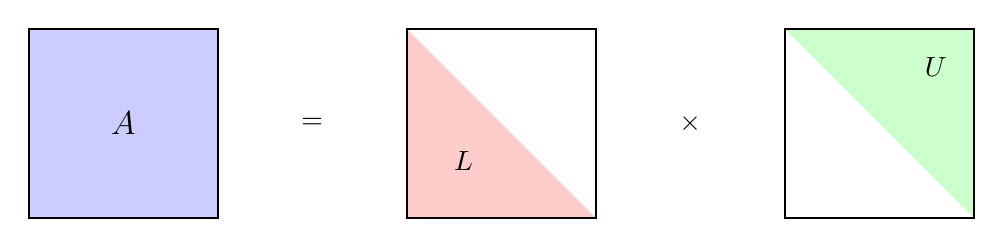
\begin{tikzpicture}[scale=1.2]

% === Matrix A ===
\draw[thick, fill=blue!20] (-4,0) rectangle (-2,2);

\node at (-3,1) {\large{$A$}};
\node at (-1,1) {$=$};

% === Matrix L ===
\begin{scope}[shift={(0,0)}]
    % Outer square
    \draw[thick] (0,0) rectangle (2,2);

    % Lower-triangular fill (red)
    \fill[red!20] (0,0) -- (0,2) -- (2,0) -- cycle;

    % Matrix outline on top
    \draw[thick] (0,0) rectangle (2,2);
\node at (0.6,0.6) {$L$};
\end{scope}

\node at (3,1) {$\times$};

% === Matrix U ===
\begin{scope}[shift={(4,0)}]
    % Outer square
    \draw[thick] (0,0) rectangle (2,2);

    % Upper-triangular fill (green)
    \fill[green!20] (0,2) -- (2,2) -- (2,0) -- cycle;

    % Matrix outline on top
    \draw[thick] (0,0) rectangle (2,2);
\node at (1.6,1.6) {$U$};
\end{scope}

\end{tikzpicture}
We won't be looking to musch in the details of how the LU decomposition is implemented. Furthermore as computer scientist (apart for those who will work on them) we won't implement this methods and we should always use the framework that has been already created.

\begin{parag}{Using a LU decomposition}
    Once the decomposition is done, how do we actually use it? We have the relation
	\begin{align*} A =  LU \end{align*}
	Therefore we found that:
	\begin{align*} x = U^{-1}\left(L^{-1}b\right) \end{align*}
	You could think like: 'but we have now to inverse of matrix to compute, this is worse!'. It would be if tose matric where some randoms ones but here we know how they behave. Those are triangular matrices. As you can try on your own those linear system are very easy to solve $\implies$ Solving a triangular system takes $O\left(n^2\right)$!
\end{parag}
\begin{parag}{Version with pivoting}
	It exists also a version with column pivoting, also known as partial pivoting:
	\begin{align*} A = PLU \end{align*}
	The way of doing it is the same but the solution is then:
	\begin{align*} x = U^{-1}\left(L^{-1}\left(P^{-1}b\right)\right) \end{align*}
	\begin{subparag}{Implementation in SciPy}
		\begin{lstlisting}[language=python]
import scipy.linalg as la 
lu, piv = la.lu_factor(A)
x = la.lu_solve((lu, piv), b)
	    \end{lstlisting}
	    
	\end{subparag}
\end{parag}


\begin{parag}{Symmetric positive definite matrices: Cholesky decomposition}
    First the definition of the symmetric matrix:
	\begin{definition}
	A matrix $A$ is \important{symmetric} if 
	\begin{align*} A = A^{T} \end{align*}
	\end{definition}
	\begin{definition}
	A symmetric matrix is \important{positive definite} if 
	\begin{align*} x^{T}Ax > 0 \;\;\; \forall \text{ nonzero }x \end{align*}
	\end{definition}
	In practice what this means is:
	\begin{itemize}
		\item No negative eigenvalues
		\item It's 'nicely behaved'
		\item It appears all the time in physics, optimization, machine learning, etc.
	\end{itemize}
	Now let's see what happen with the LU decomposition but when we are with a symmetric matrix:
	\begin{align*} A = LU \end{align*}
	Which implies directly:
	\begin{align*} A = LU = \left(LU\right)^{T} = U^{T}L^{T} \end{align*}
	So we have two relations $A =  LU$ and $A = U^TL^T$ since factorization of a matrix are unique for triangular factors, that menas the left hand and right hand factos must match. So we must have:
	\begin{align*} L = U^T  \text{ and } U =  L^T\end{align*}
	Therefore:
	\begin{align*} A = LL^T \end{align*}
	Where $L$ is lower triangular with \important{positive} diagonal entries.\\
	This is great! We only need to store one matrix instead of two, we saved half of the storage.
	For instance given:
	\begin{align*} \begin{pmatrix} A_{11} & A_{21} \\ A_{21} & A_{22} \end{pmatrix} = \begin{pmatrix} L_{11} & 0 \\ L_{21} & L_{22} \end{pmatrix} \begin{pmatrix} L_{11} & L_{21} \\ 0 &  L_{22}\end{pmatrix} \end{align*}
	We have that:
	\begin{align*} 
		L_{11} &= \sqrt{A_{11}}\\
		L_{21} &= \frac{A_{21}}{L_{11}}\\
		L_{22} &= \sqrt{A_{22} - L_{21}^2}
	\end{align*}
	
\end{parag}







